%!TEX root = ../../Paper.tex
\chapter{Trend Analysis on Twitter: Detected Trends}
\label{cha:trend-stories}

\section{Detected Trends - Overview}
\label{sec:trend-overview}

By using our tool, we collected and analyzed about 18 million English tweets from the USA between 15th of December 2014 and 15th of January 2015. In this period of time, we were able to detect several major events such as Christmas and New Year, the Sony Hack concerning the movie \enquote{The Interview}, the PSN Hack, the Air Asia plane crash and the attack on Charlie Hebdo. Figure \ref{fig:major-trend-overview} compares three major events in this time frame based on the number of occurrences of popular hashtags. 

\begin{figure}[H]
  \centering
        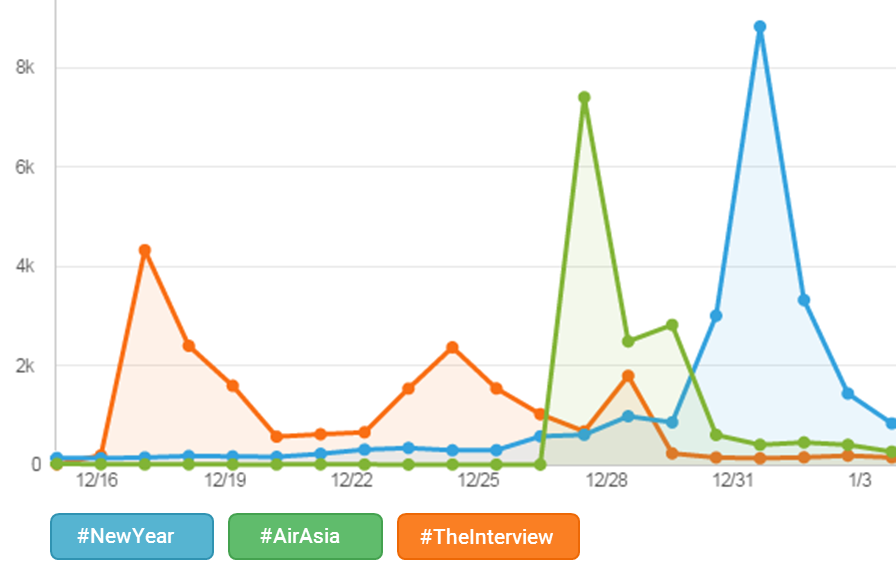
\includegraphics[width=\textwidth]{final_major_trend_overview}
  \caption[Detected Twitter Trends in December 2014]{Detected Twitter Trends in December 2014}
  \label{fig:major-trend-overview}
\end{figure}

In the following sections, we will analyze and present some of these trends in more detail aiming to get high-quality insights. 

\section{New Year on Twitter}
\label{sec:happy-new-year}
The most obvious events that occurred in our analysis period was Christmas and New Year. Both trends are compared in figure \ref{fig:christmas-new-year-time-series}. The number of tweets mentioning Christmas already started to rise many days before Christmas Eve probably because of Advent and Christmas preparations. In contrast, the trend of New Year lasted only for about four days, but with a much higher peak on New Year Eve.

\begin{figure}[H]
  \centering
        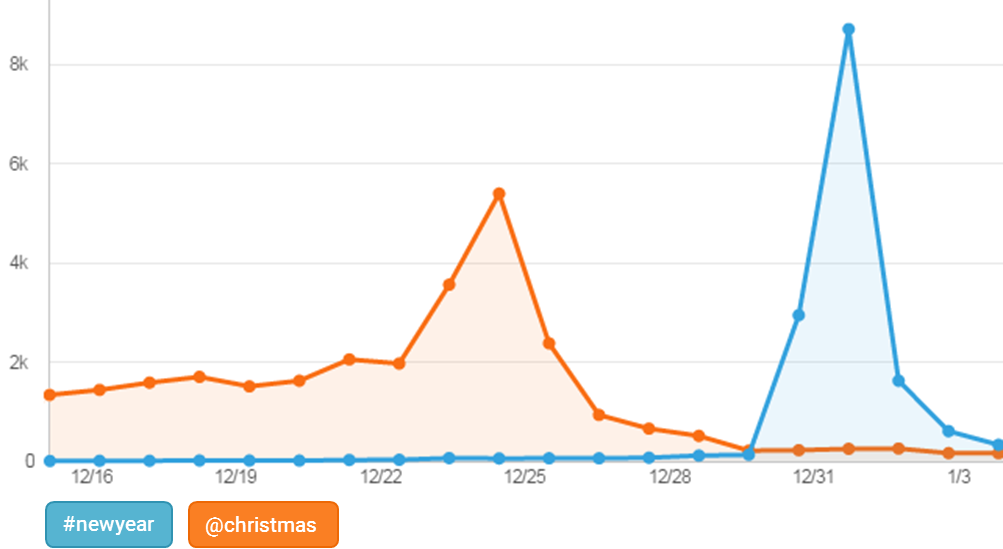
\includegraphics[width=\textwidth]{final_timeseries_newyear}
  \caption[Time Series - Christmas \& New Year ]{Time Series - Christmas \& New Year}
  \label{fig:christmas-new-year-time-series}
  \vspace{-1.3em}
\end{figure}

Based on the rapid increase of tweets mentioning the New Year in a short period, we could detect several hashtags related to this event. Following hashtags were discovered as being the main used ones:

\begin{figure}[H]
\begin{multicols}{3}
  \begin{itemize}[label={}]
  \item \#newyear
  \item \#newyearseve
  \item \#nye
  \item \#hny
  \item \#goodbye2014
  \item \#bye2014
  \item \#nye2015
  \item \#midnight
  \item \#ihatenewyears
  \item \#newyearseveproblems
  \item \#newyear2015
  \item \#happynewyear
  \item \#hello2015
  \item \#welcome2015
  \item \#hi2015
  \item \#newyears
\end{itemize}
\fixspacing
\end{multicols}
\caption*{Listing 4.1: New Year Hashtags and User Mentions}
\captionlistentry[lstlisting]{New Year Hashtags and User Mentions}
\end{figure}

The word cloud depicted in figure \ref{fig:new-year-word-cloud} illustrates the most frequent used words from our dataset related to the New Year.

\begin{figure}[H]
  \centering
        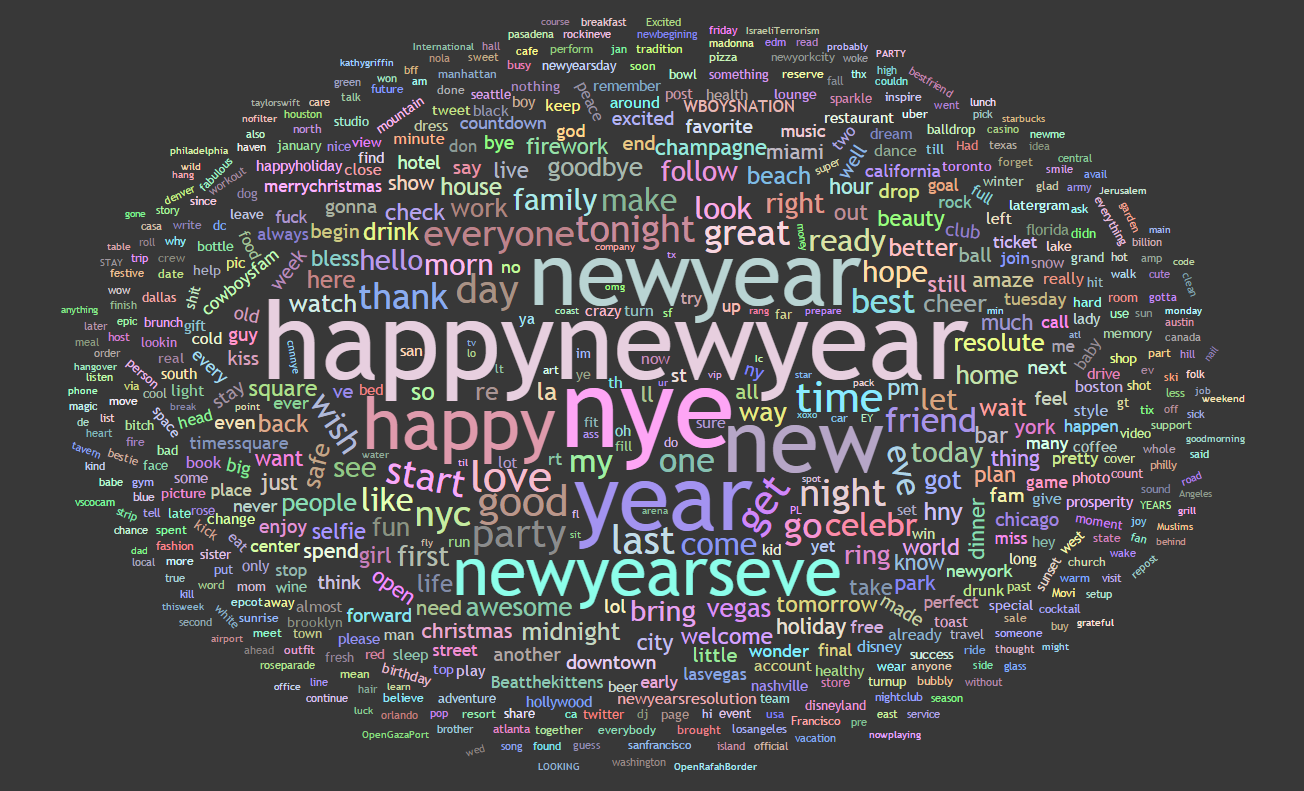
\includegraphics[width=\textwidth]{final_wordcloud_newyear}
  \caption[Word Cloud - New Year Eve]{Word Cloud - New Year Eve}
  \label{fig:new-year-word-cloud}
  \vspace{-1.3em}
\end{figure}

Figure \ref{fig:new-year-heat-map} shows a geospatial comparison of the activity of tweets mentioning the New Year during  two different points in time. The left heat map shows the west coast few minutes after midnight on 1st January 2015 (Timezone: UTC-08). In contrast, the right map visualizes the same Twitter activity three hours before on the east coast (Timezone: UTC-05). It is clearly recognizable that the New Year midnight in each time zone generates a huge amount of content related to this event in a short period of time.

\begin{figure}[H]
  \centering
        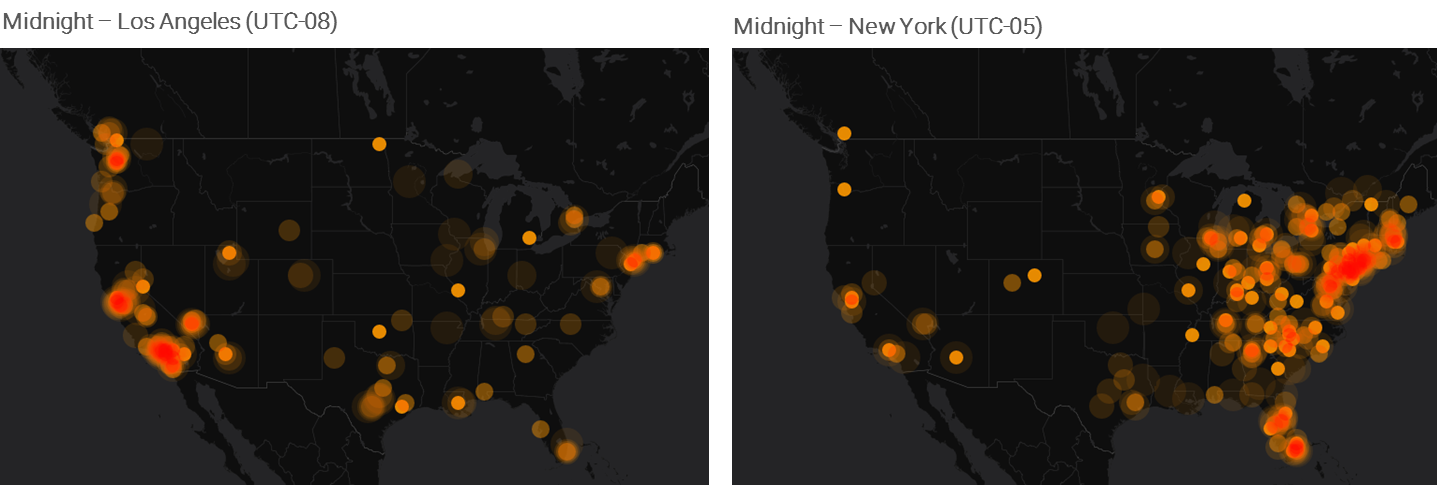
\includegraphics[width=\textwidth]{final_geospatial_newyear}
  \caption[Geospatial Comparison - New Year Eve]{Geospatial Comparison - New Year Eve}
  \label{fig:new-year-heat-map}
  \vspace{-1.3em}
\end{figure}

Besides the preceding analysis of the geolocation and spreading of this trend, we analyzed the sentiment of the American people regarding the New Year as shown in figure \ref{fig:new-year-sentiment}. Thereby, the majority of tweets contains positive or at least neutral opinions and only a small number has a negative attitude.

\begin{figure}[H]
  \centering
        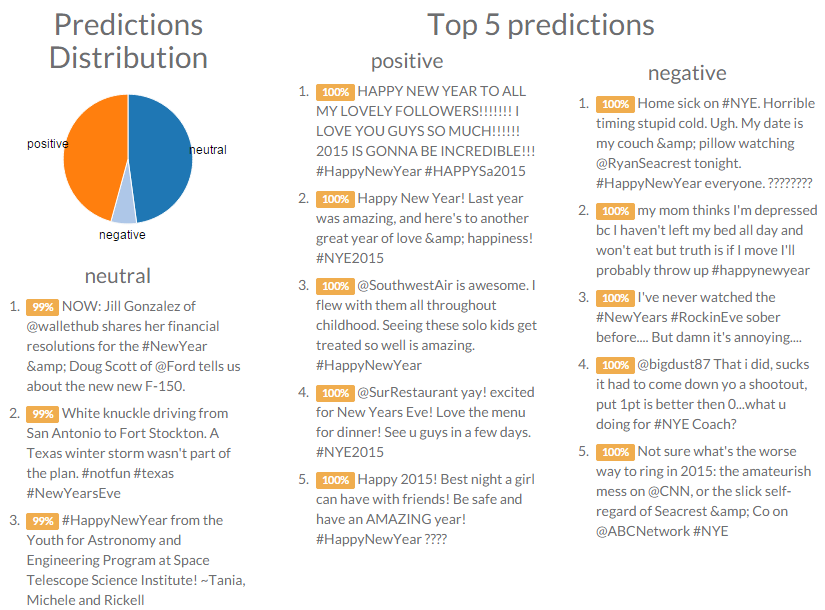
\includegraphics[width=\textwidth]{final_sentiment_newyear}
  \caption[Sentiment - New Year Eve]{Sentiment - New Year Eve}
  \label{fig:new-year-sentiment}
  \vspace{-1.3em}
\end{figure}


\section{Air Asia Flight Tragedy}
\label{sec:air-asia-flight-tragedy}
On 28\textsuperscript{th} of December a terrible tragedy hit the news: a plane from the Air Asia carrier (QZ8501) crashed into the Java sea between Indonesia and Singapore. On board of the flight were 162 people on their way from Surabaya in Indonesia to Changi Airport in Singapore. It was around 06:12 local time when the pilot contacted air traffic control to request a change in flight altitude in order to prevent being caught by the storm clouds which are typical for that area. Air traffic control gave the permission to do so a few minutes later, but could not reach the plane anymore \cite{bbc2014flight}. The plane had already crashed into the sea. Many people related this event to the tragedy of flight MH370 from Malaysia Airlines, which got lost on March 8\textsuperscript{th}, 2014 \cite{nbc2014by} after the missing of flight QZ8501 was announced.

Figure \ref{fig:air-asia-time-series} illustrates the impact of this tragedy on Twitter with two distinguishable peaks on 28\textsuperscript{th} of December, after it was first announced that the plane is missing, and on the 30\textsuperscript{th} of December, after the first wreckage was found. As of now, the recovery effort is still ongoing as well as the discussion of this event on Twitter.

\begin{figure}[H]
  \centering
        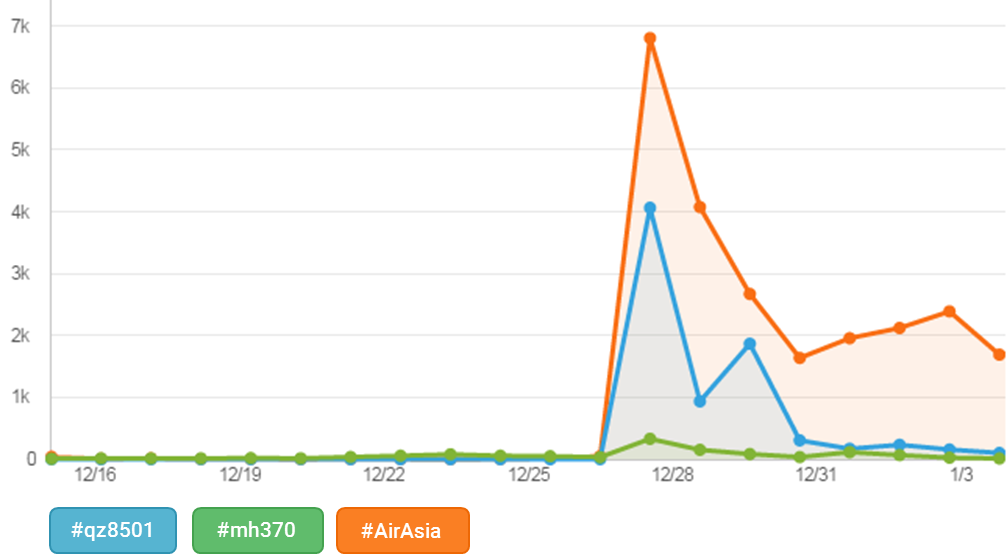
\includegraphics[width=\textwidth]{final_timeseries_airasia}
  \caption[Time Series - AirAsia Tragedy]{Time Series - AirAsia Tragedy}
  \label{fig:air-asia-time-series}
  \vspace{-1.3em}
\end{figure}

Our Early Trend Detector was able to identify the following list of related hashtags used by Twitter users to discuss this news or to express griefs and sympathy with the families and relatives:

\begin{figure}[H]
\begin{multicols}{2}
\begin{itemize}[label={}]
	\item \#airasia
	\item \#qz8501
    \item \#prayforairasia
    \item \#prayforqz8501
    \item \#airasia8501
    \item \#mh370
\end{itemize}
\end{multicols}
\caption*{Listing 4.2: Air Asia Hashtags and User Mentions}
\captionlistentry[lstlisting]{Air Asia Hashtags and User Mentions}
\end{figure}

As mentioned earlier, many people related the crash of Air Asia flight QZ8501 with the disappearance of the Malaysia Air flight MH370. That explains why both flight numbers are trending topics.

\begin{figure}[H]
  \centering
        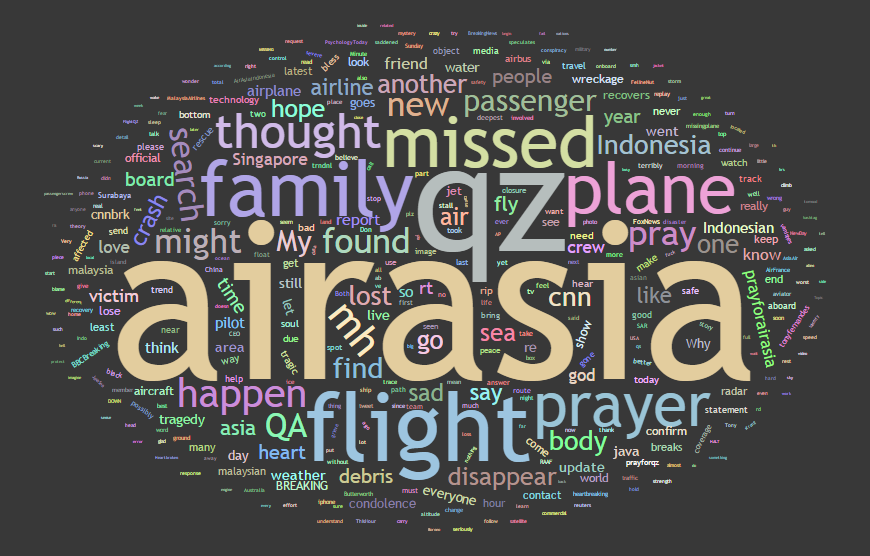
\includegraphics[width=\textwidth]{final_wordcloud_airasia}
  \caption[Word Cloud - AirAsia Tragedy]{Word Cloud - AirAsia Flight Tragedy}
  \label{fig:air-asia-flight-tragedy-word-cloud}
  \vspace{-1.3em}
\end{figure}

The word cloud in figure \ref{fig:air-asia-flight-tragedy-word-cloud} visualizes the most commonly used words in tweets about the plane crash. A hypothesis based on the word cloud is that the tweets have two different topics. One topic is news (discussion about the tragedy) and the other topic is emotional (showing of condolence to the families of the victims).
We extracted tweets from our dataset related to this event and used LDA for topic modeling in order to further analyze our hypothesis. These topics are presented in listing \ref{lst:topic-model-air-asia}.

\begin{lstlisting}[caption={[Topic Model for Air Asia Flight Tragedy] Topic Model for Air Asia Flight Tragedy}, label={lst:topic-model-air-asia}, float=h]
	airasia (139) missing (76) flight (55) air (39) indonesia (37) singapore (33) asia (31) °\DNumber°

	airasia (126) missing (60) planes (50) find (39) plane (36) world (20) technology (15) °\DNumber°

	prayers (86) families (81) thoughts (72) airasia (24) crash (14) thought (12) airfrance (8) °\DNumber°

	cnn (13) put (7) speculation (6) ground (6) airasia (6) speed (5) stop (5) °\DNumber°

	airasia (140) found (65) plane (53) sea (51) bodies (49) search (49) debris (40) °\DNumber°

	airasia (146) flight (122) amp (99) happened (87) disappearance (14) malaysia (7) trends (6) °\DNumber°

	airasia (257) families (144) flight (90) passengers (69) prayers (58) amp (47) missing (39) °\DNumber°

	airasia (35) weather (23) flight (17) pilots (13) fly (12) bad (12) path (10) °\DNumber°

	raaf (8) butterworth (8) china (8) australia (5) russia (5) trndnl (5) trending (5)
\end{lstlisting}

We used LDA to model nine different topics showing the 7 most relevant words of each topic. There is an observable difference between reporting tweets (like topic 0, 1, 4 and 7) and emotional tweets (like topic 2 and 6). Topics 3 and 8 stand out from the other, topic 3 is about the famous news network CNN, which was one of the first to bring coverage about the crashed plane. Topic 8 on the other hand is about RAAF Butterworth airport in Malaysia, this airport is used by Australia and others to coordinate the search for the missing wreckage of the airplane.
This shows that our initial hypothesis is true. There are two different subjects tweeting about the airplane crash of flight QZ8501.

The sentimental analysis of Air Asia related tweets in figure \ref{fig:air-asia-sentiment} shows a significant difference compared to the sentiment of New Year Eve in figure \ref{fig:new-year-sentiment}. Only a small portion of tweets is classified as positive, mostly containing words of hope, compassion and prayer. A larger portion of tweets are labeled with a negative sentiment by people referencing this terrible tragedy and condemning the end of this year. The biggest portion of tweets contains neutral information such as objective news updates and discussion.

\begin{figure}[H]
  \centering
        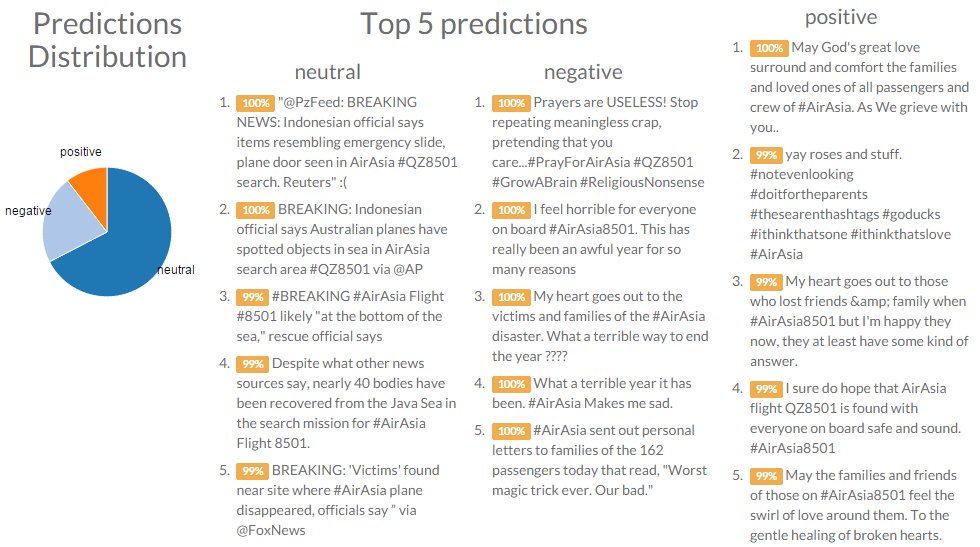
\includegraphics[width=\textwidth]{final_sentiment_airasia}
  \caption[Sentiment - AirAsia Tragedy]{Sentiment - AirAsia Tragedy}
  \label{fig:air-asia-sentiment}
  \vspace{-1.3em}
\end{figure}

\subsubsection{Comparison with Google Trends}
In this section, we compare the trend data related to the Air Asia tragedy with statistics from Google Trends to check for similarities and the validity of detecting trends on Twitter based on a small statistical sample. Further, we want to get additional insights in the character of Twitter trends and how close those trends resemble real world activities. Google Trends makes it possible to analyze the search-volume for specified search terms entered in the Google Search. Kwak et al. argue that search keywords from Google \enquote{represent topics users are interested in and popular keywords represent hot trends} \cite[6]{kwak2010what}. Therefore, those keyword trends \enquote{have become a good indicator to understand activities in the real world} \cite[6]{kwak2010what}.

Figure \ref{fig:google-trends-comparison-timeseries} illustrates the comparison between the time series visualization of the Air Asia flight tragedy on Twitter and a Google Trends statistic for similar search terms. 

\begin{figure}[H]
  \centering
        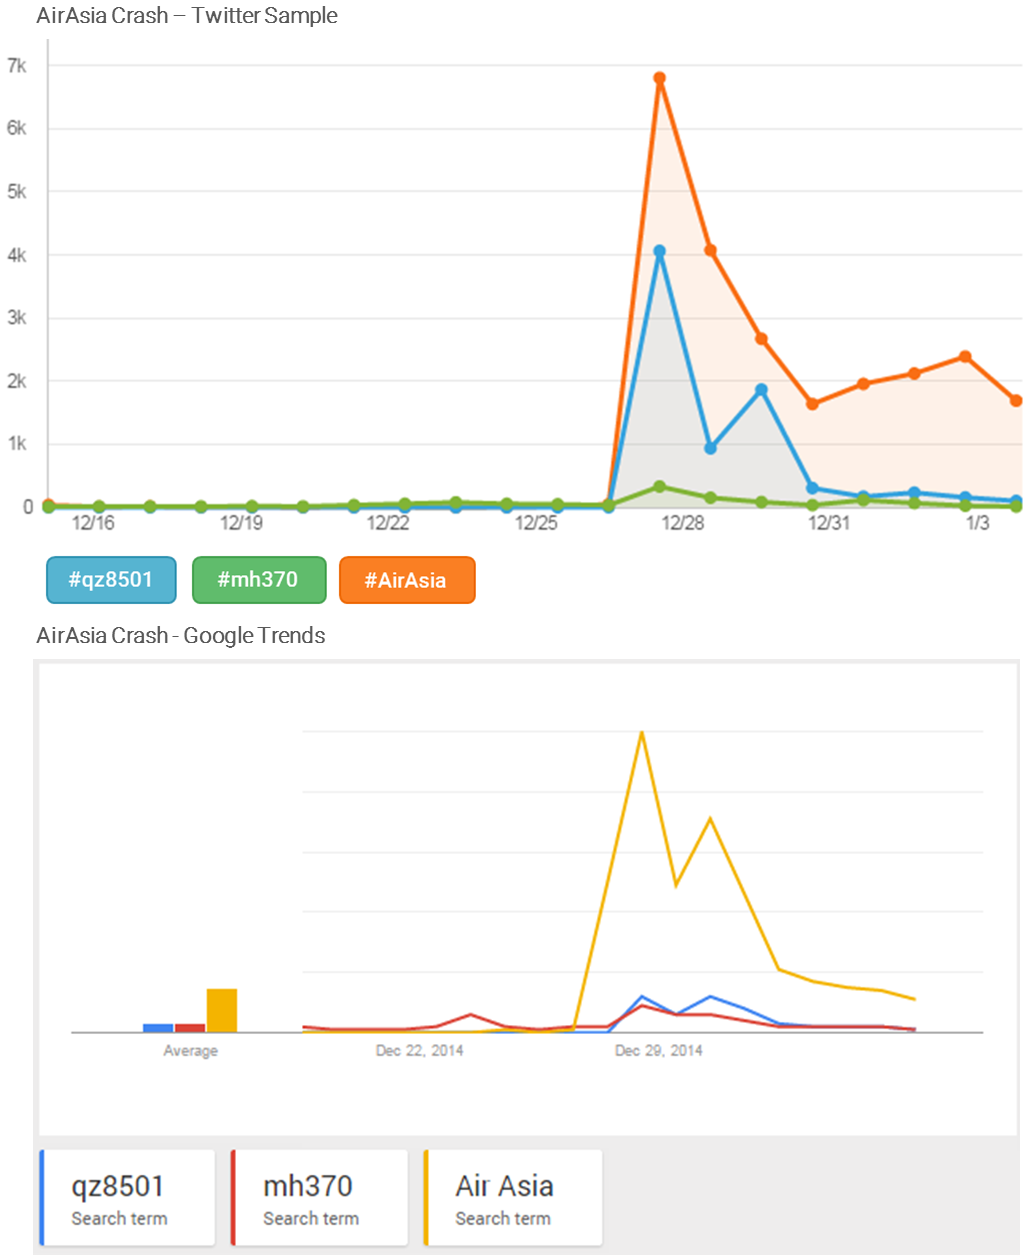
\includegraphics[width=\textwidth]{final_googletrend_timeseries_comparison_airasia}
  \caption[Time Series - Comparison with Google Trends]{Time Series - Comparison with Google Trends}
  \label{fig:google-trends-comparison-timeseries}
  \vspace{-1.3em}
\end{figure}

There is a clear resemblance between the trend curve based on our dataset of tweets and the curve on Google Trends for the used search terms. Moreover, figure \ref{fig:google-trends-comparison-geospatial} compares the regional interest about the Air Asia tragedy in the US on Twitter with the relative search volume for each state on Google Search. 

\begin{figure}[H]
  \centering
        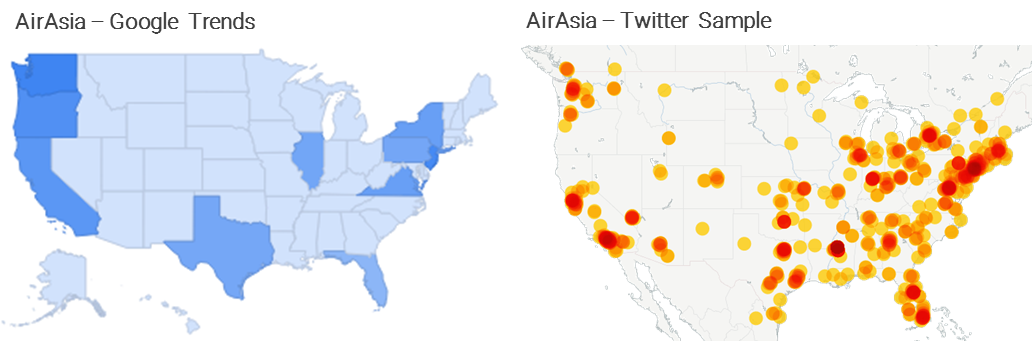
\includegraphics[width=\textwidth]{final_googletrend_regional_comparison_airasia}
  \caption[Geospatial - Comparison with Google Trends]{Geospatial - Comparison with Google Trends}
  \label{fig:google-trends-comparison-geospatial}
  \vspace{-1.3em}
\end{figure}

Both comparisons demonstrate a high similarity between Twitter trends and Google Search trends. We conclude that detecting and analyzing Twitter for trends provides high-quality insights into the world’s interest in global events. Twitter trends even resemble regional interests in certain topics with a high accuracy. Further, Twitter is one of the fastest ways to detect and predict global trends, due to its open access to real-time data. However, Kwak et al. mentions that interactions such as retweet and reply \enquote{might be a factor to keep trending topics persist} for a longer time on Twitter.

\section{Gaming Network Outage}
\label{sec:christmas-network-outage}
On the 24\textsuperscript{th} of December in 2014, hackers started to attack the Playstation Network (PSN) and the Microsoft Xbox Live Network. The hacker attacks brought the networks down for several days. The gamer community was outraged not to be able to play games during this period of time \cite{wool2014sony}. After a few days, a hacker group called Lizard Squad claimed credit for the attack. In the end, the popular german internet entrepreneur Kim Dotcom paid Lizard Squad with vouchers for his web platform \textit{MEGA} \cite{Dotcom2014}. In return, Lizard Squad decided to stop further attacks on the gaming networks. After the network recovered, Sony announced to give discounts to PSN users as a compensation. Figure \ref{fig:christmas-network-outage-time-series} shows how the Twitter activity regarding this topic increased rapidly during the period of attacks.

\begin{figure}[H]
  \centering
        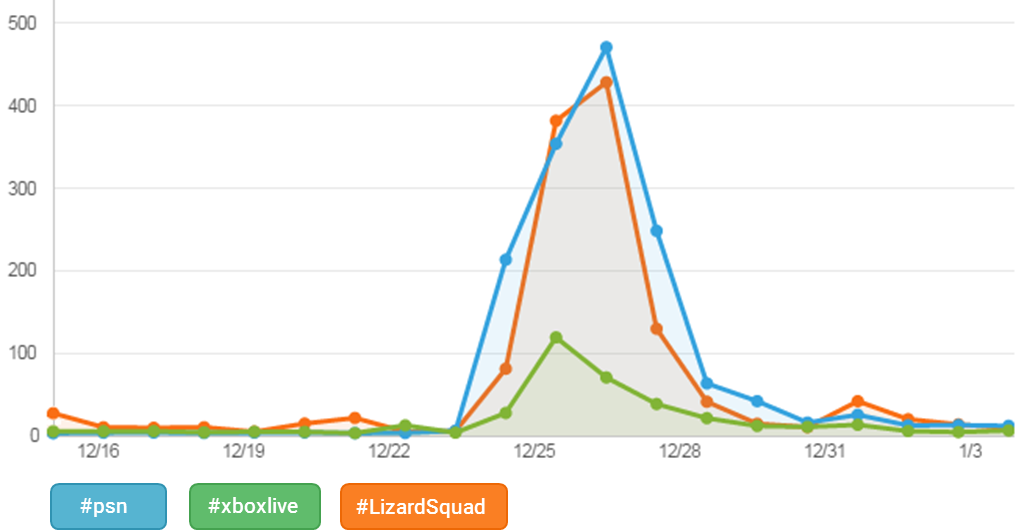
\includegraphics[width=\textwidth]{final_timeseries_psnhack}
  \caption[Time Series - Gaming Network Outage]{Time Series - Gaming Network Outage}
  \label{fig:christmas-network-outage-time-series}
  \vspace{-1.3em}
\end{figure}

The involved persons and topics are reflected in the following list of hashtags and user mentions that we were able to identify for this trend:

\begin{figure}[H]
\begin{multicols}{3}
\begin{itemize}[label={}]
	\item \#finestsquad
	\item \#lizardpatrol
    \item \#lizardsquad
    \item \#payingfornothing
    \item \#playstationnetwork
    \item \#playstationsucks
    \item \#psn
    \item \#psndown
    \item \#PSNDownTime
    \item \#psnup
    \item \#xboxlivedown
    \item \#xboxsupport
    \item @AskPlayStation
    \item @KimDotcom
    \item @LizardMafia
    \item @MEGAprivacy
    \item @PlayStation
\end{itemize}
  \fixspacing
\end{multicols}
\caption*{Listing 4.4: Gaming Network Outage Hashtags and User Mentions}
\captionlistentry[lstlisting]{Gaming Network Outage Hashtags and User Mentions}
\end{figure}

We fetched tweets containing at least one of the listed hashtags or user mentions and created a word cloud, depicted in figure \ref{fig:christmas-network-outage-word-cloud}.

\begin{figure}[H]
  \centering
        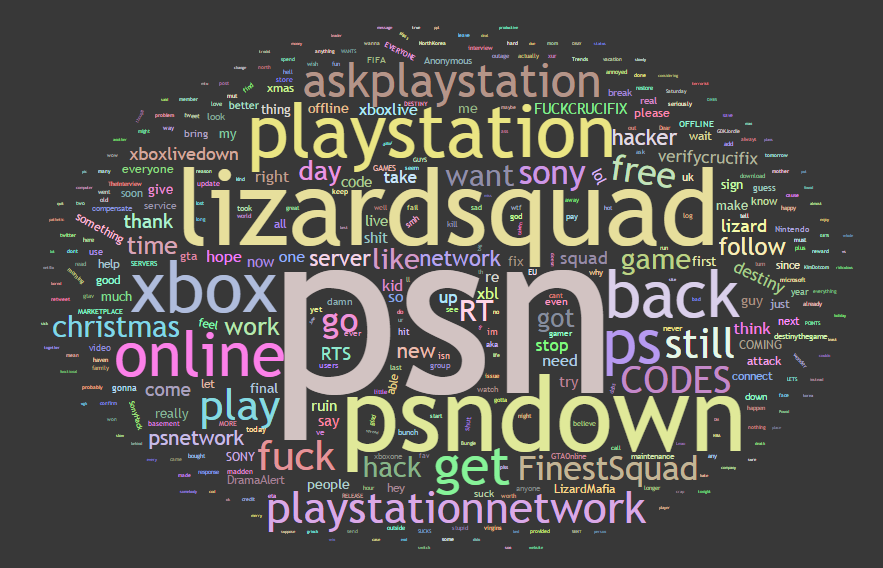
\includegraphics[width=\textwidth]{final_wordcloud_psnhack}
  \caption[Word Cloud - Gaming Network Outage]{Word Cloud - Gaming Network Outage}
  \label{fig:christmas-network-outage-word-cloud}
  \vspace{-1.3em}
\end{figure}

In the next step, we wanted to find out which of the words in the word cloud are used together most of the time. Therefore, we performed topic modeling on the trend related tweets by using LDA.
The identified topics are displayed in listing \ref{lst:topic-model-network}.

\begin{lstlisting}[caption={[Topic Model for Christmas Network Outage] Topic Model for Christmas Network Outage}, label={lst:topic-model-network}, float=h]
	xbox (101) playstation (50) watch (44) movie (32) fuckcrucifix (31) north (29) korea (27) interview (27) °\DNumber°

	xbox (310) christmas (178) play (81) xboxlivedown (72) live (71) xboxlive (68) xboxsupport (66) day (63) °\DNumber°

	playstation (55) dollar (27) psn (20) company (19) lizardsquad (18) sony (17) billion (16) multi (12) °\DNumber°

	fuckcrucifix (204) lizardmafia (172) lizardsquad (125) fuck (116) lizard (108) squad (102) finestsquad (95) stop (94) °\DNumber°

	psn (468) back (461) playstation (324) online (246) askplaystation (205) network (173) psndown (89) working (88) °\DNumber°

	xbox (250) psn (230) sign (215) connect (143) live (110) error (103) account (93) issues (82)
\end{lstlisting}

The words that were clearly visible in the word cloud are also dominating the detected topics. Furthermore, the detected topics reflect the real events in a reasonably good way.

Topic 1 covers words indicating a discussion about a connection between the DDoS attack during Christmas and a previous hack against Sony concerning the movie ‘The Interview’ \cite{bbc2014the}. The second topic is about the hack affecting the Xbox Live Network. Obviously, a lot of people tweeted to Microsoft's support. Topic 5 is similar to topic 2, however, these terms are related to the Playstation Network. Topic 6 covers general terms concerning the hack and the instability to connect to the networks or to play a game. Topic 4 is focused on terms about Lizard Squad. The words indicate that the gamer community was not very amused about the hack. Topic 3 contains terms about the financial impact of such a hack and the claim for redemption for the lost hours of not being able to use the networks.

Figure \ref{fig:network-outage-sentiment} displays the sentiment of the user community regarding the gaming consoles and their hacks. Obviously, some people were quite upset. Interestingly, the anger was directed against the companies and not against the hacker group. Some people, however, were thankful for the past year and backed up Sony and Microsoft.

\begin{figure}[H]
  \centering
        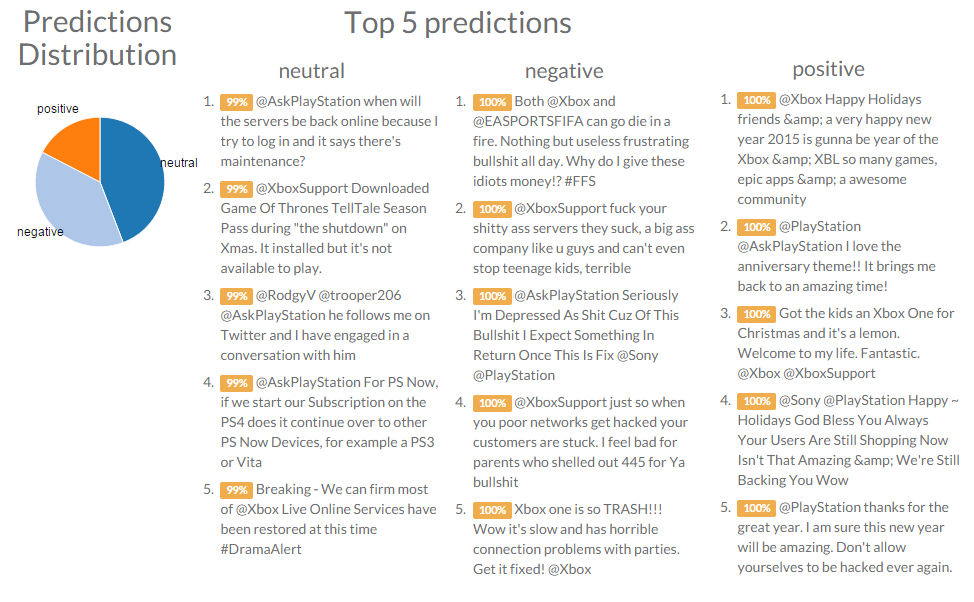
\includegraphics[width=\textwidth]{final_sentiment_psnhack}
  \caption[Sentiment - Gaming Network Outage]{Sentiment - Gaming Network Outage}
  \label{fig:network-outage-sentiment}
  \vspace{-1.3em}
\end{figure}